\section{Results}
% \vspace{-1.5mm}
\subsection{Overall Results}
The overall results of our experiments are shown in Table \ref{results}. First, our model SCCL achieves ACCs of 79.20\%, 80.05\%, 80.24\%, 78.36\%, 79.00\%, and 78.55\% in Order 1-6, respectively, which are 2.37\%, 0.9\%, 0.66\%, 3.28\%, 2.49\%, and 2.40\% higher than the second-best performance of the continual learning baselines. 
It shows that the performance of the continually learned model is well-maintained in SCCL, but the  problem of CF still exists. SCCL achieves state-of-the-art ACCs compared with the baseline models, indicating the effectiveness of our proposed framework. We also observe that the performance variance is small in the SCCL model for different orders, which implies that our models are not sensitive to the order of task sequences. 

Second, the results of BWT range from -3.75\% to 0.57\% in SCCL for Orders 1-6, which demonstrates knowledge forgetting during the continual learning procedure. The results of SCCL are relatively higher than CE-based models, indicating that SCCL suffers from a milder impact of CF.   Note that  the BWT of SCCL is 0.57\% in  Order 4, which indicates that SCCL can even backward transfer the knowledge from the current tasks to previous tasks. But compared with CL-LwF, CL-MAS, and CL-EWC, the values  of ACCs in SCCL are higher, but BWTs are adverse.  It implies that using the regularization-based strategies, the fine-tuning performance is destructed for explicit control of representations. In this way, BWTs become low since the fine-tuning performance on downstream tasks is relatively weak. 


 
\begin{figure*}
    \centering
    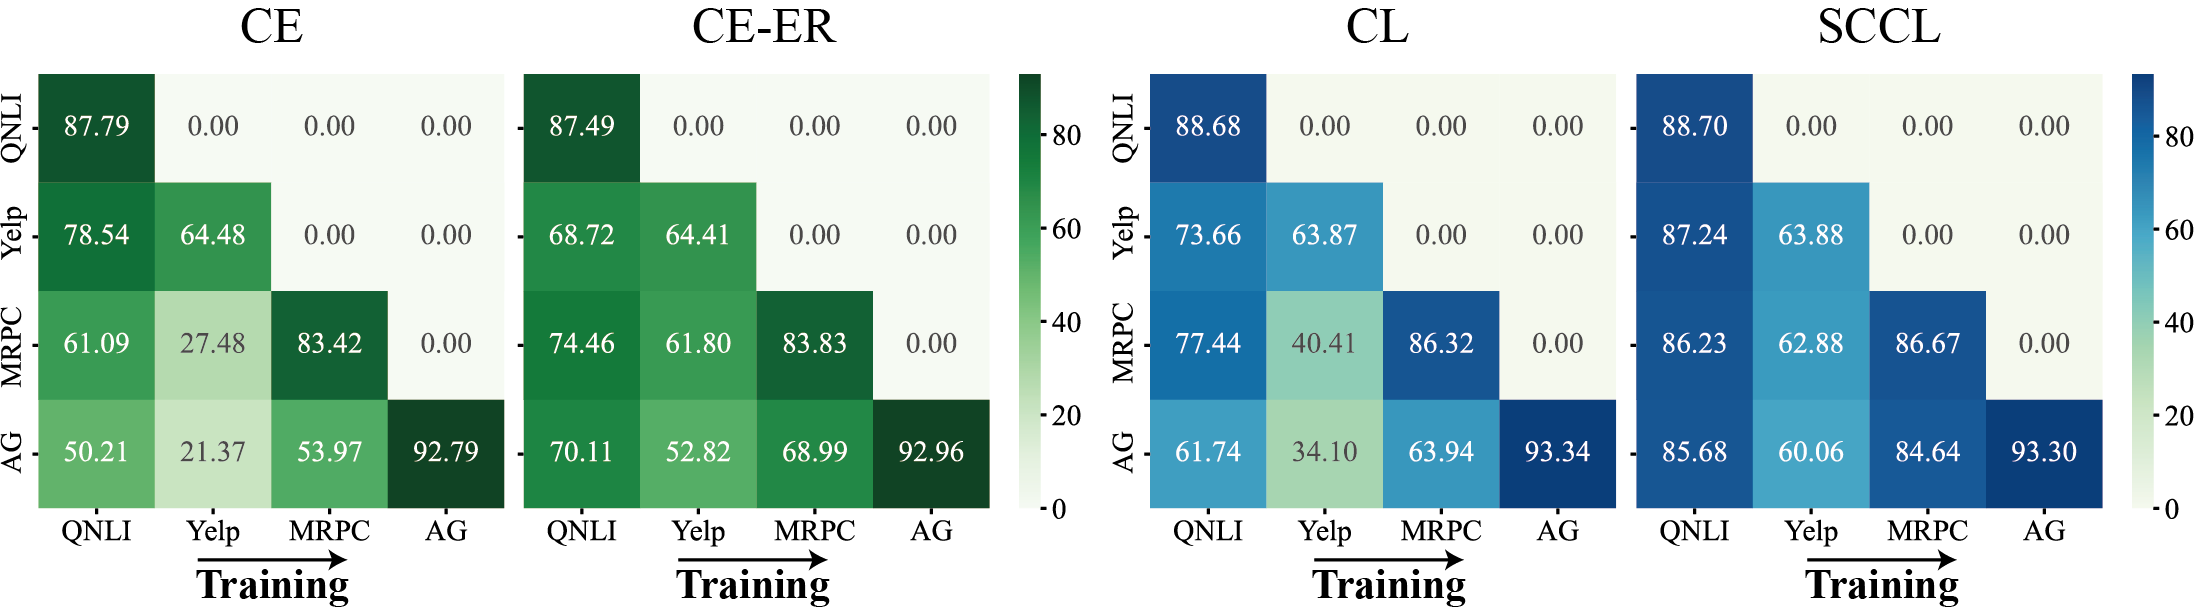
\includegraphics[width=\hsize]{detailed.png}
    \caption{Detailed results during continual learning procedure for different strategies in Order 3.}
    \label{details}
    \vspace{-5mm}
\end{figure*}

\begin{figure}[pt]
    \centering
    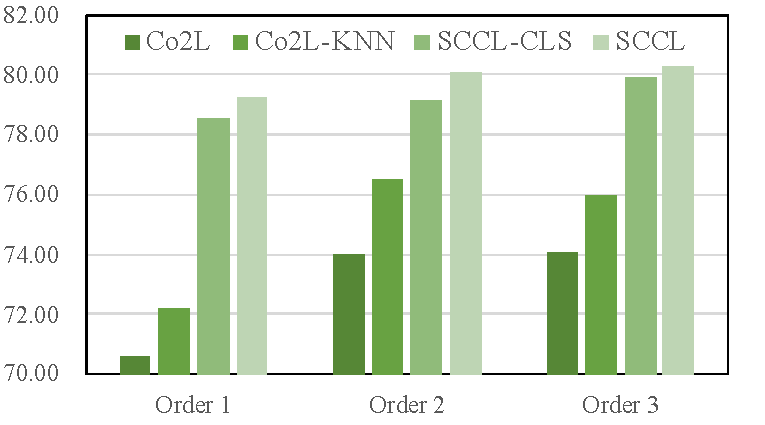
\includegraphics[width=0.87\hsize]{Ablation.pdf}
    \caption{Comparisons of SCCL and Co$^2$L with ablation studies.}
    \label{abl}
    \vspace{-6mm}
\end{figure} 

Third,  the  extended CL-based models achieve stronger performance than corresponding standard CE-based models. For example,  the model CL-LwF achieves 
ACCs of 76.53\%, 79.15\%, 79.58\%, 68.24\%, 72.39\%, and 71.48\%, which are 4.44\%, 7.02\%, 6.04\%, 0.01\%, 9.24\% and 3.56\% higher than those of CE-LwF. The results of CL, CL-MAS, and CL-EWC are in a similar pattern.  The results reflect that contrastive learning with a kNN classifier for continual learning has a stronger ability to overcome CF. But we observe that Co$^2$L achieves relatively low performance compared with our model, which proves that Co$^2$L is not effective for task-incremental learning. It can be explained that Co$^2$L keeps the knowledge of classes and separate the tasks with clear boundary, by using asymmetric supervised contrastive loss, which makes it difficult to distinguish a representation for different task purposes.


Finally, we observe a significant variance in the results of different task orders for regularization-based methods. For example, ACCs of CL-EWC range from 75.89\% to 66.74\%.  But in CE-ER or SCCL the variance is less drastic, such as CE-ER ranging from 76.90\% to 75.08\% and SCCL ranging from 80.24\% to 78.55\%. The phenomenon may result from that knowledge forgetting of previous tasks increases step by step for information los, but no samples help recover such information in regularization-based methods.


% \vspace{-mm}
\subsection{Ablation Study}
We show the ablation study of memory replay and IRD in the last two rows in Table 2. The ACCs of the models w/o memory replay range from 71.22\%, to 80.27\% for Order 1-6,  which are 2.01\%, 1.42\%, -0.03\%, 2.71\%, 7.78\%, and 3.91\% lower than SCCL, respectively.  It shows the effectiveness of memory replay, without which ACC also becomes less robust to task orders. Then ACCs of the models w/o IRD are 1.63\%, 0.32\%, 0.76\%, 4.49\%, 2.11\%, and 4.23\% lower than SCCL for Order 1-6, respectively. We observe that the models w/o IRD are more robust to task orders, which implies that rehearsal-based methods  are less sensitive to task sequences. Comparing the model w/o IRD with CE-ER, the model performance are also higher than those of CE-ER, which uses almost the same training strategy. The phenomenon demonstrates the effectiveness of contrastive learning in overcoming CF.

We also compare our model with Co$^2$L in ablation studies (Figure \ref{abl}). First, we replace the kNN module of SCCL with a decoupled linear classifier like \cite{cha2021co2l} (SCCL-CLS), where ACCs are slightly smaller than SCCL. It indicates that the kNN module in SCCL can achieve satisfactory performance without additional training on the final representations of contrastive learning. Then we replace the decoupled linear classifier of Co$^2$L with our kNN module (Co$^2$L-kNN), and we observe an increase in performance. It implies that the representations learned by  Co$^2$L are not separated clearly in the feature space, thus a trained linear layer is less effective for classification. But K-means selection of the samples and kNN inference module can estimate the representation distribution more precisely, resulting in better performance. Note that the results of  SCCL are also stronger than Co$^2$L-kNN, which indicates the effectiveness of our model on task-incremental continual learning.


 \begin{figure*}
    \centering
    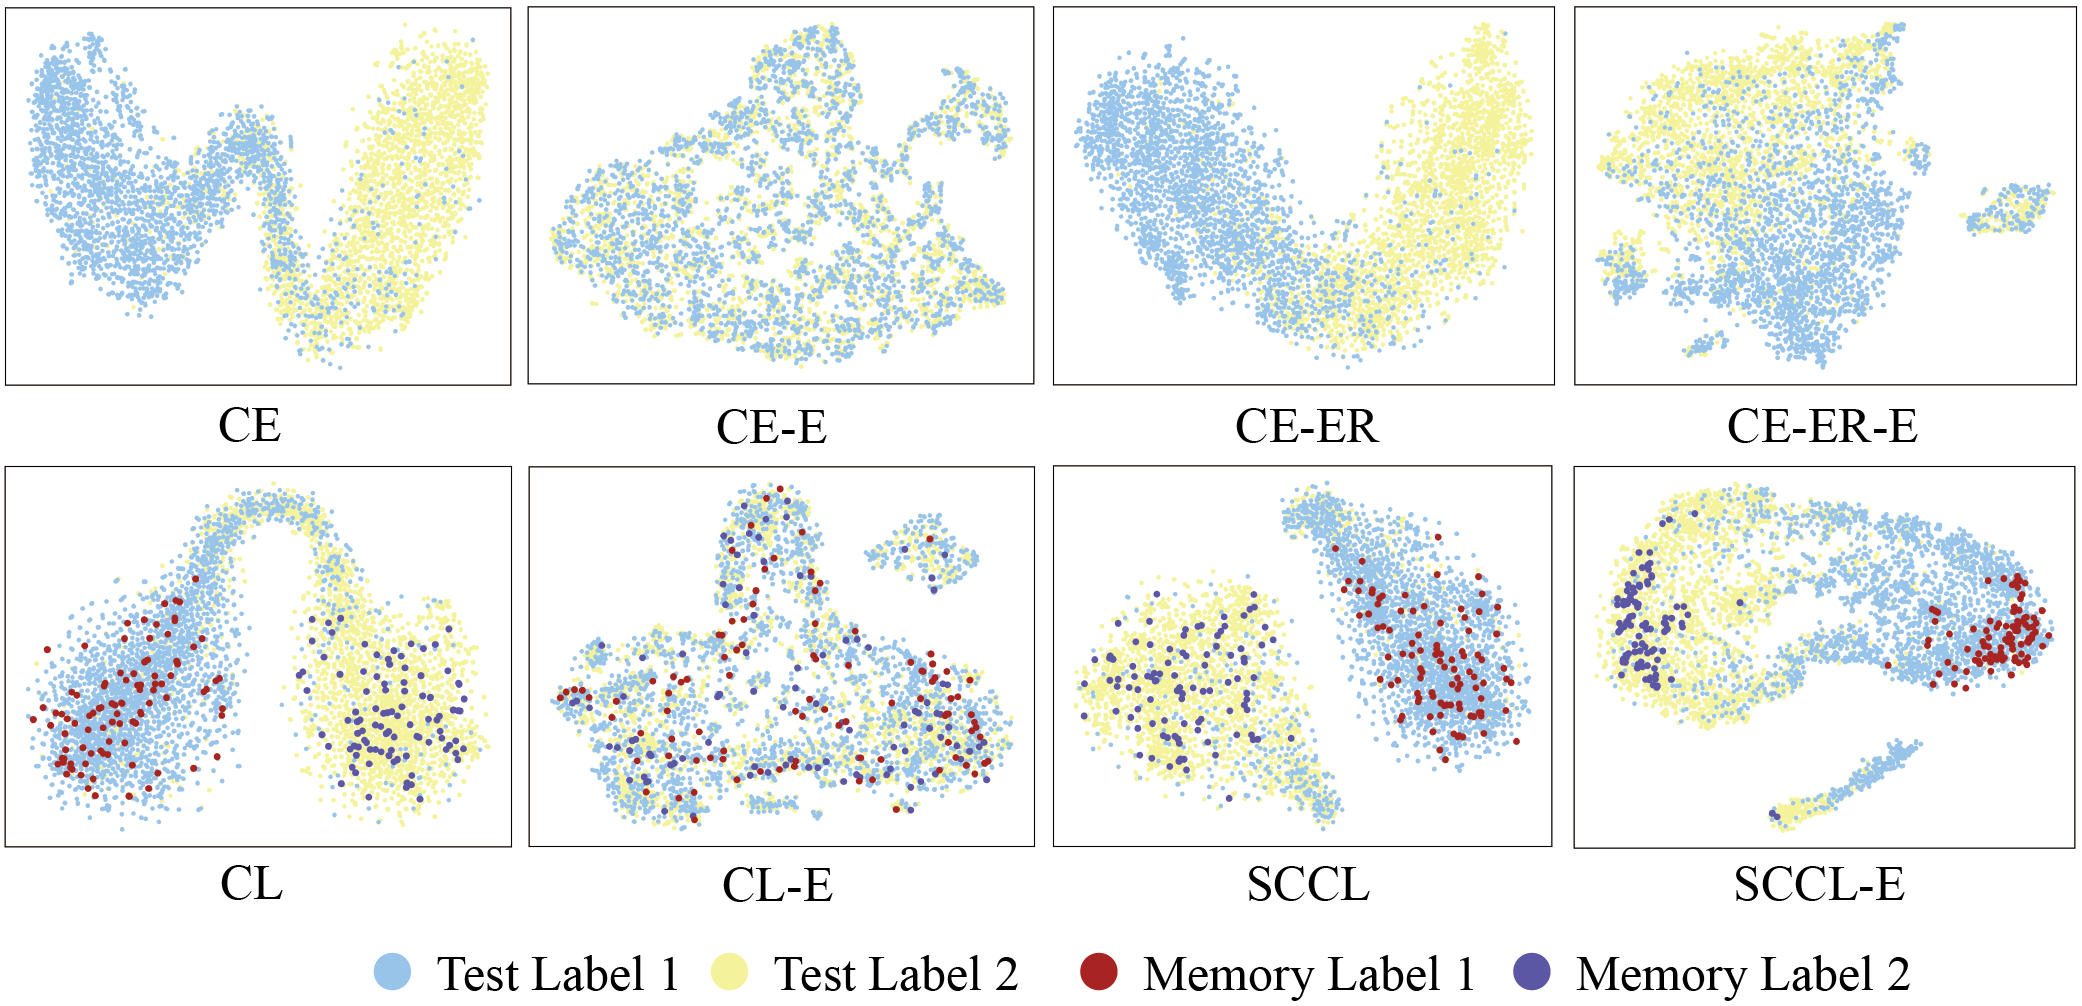
\includegraphics[width=0.9\hsize]{2.png}
    \caption{t-SNE visualization of the representations of QNLI samples learned based on the different continual learning methods in Order 5. `E' refers to the representations at the end of continual learning.}
    \label{vis}
        \vspace{-5mm}
\end{figure*}

\subsection{Detailed Results}
As an example, we show the detailed results of Order 3 in several models (Figure \ref{details}). 
First, in the model of CE, we observe that the test accuracies of QNLI decrease from 87.78\% to 50.21\% step by step with the continual training on the task QNLI, Yelp, MRPC, and AG. The accuracies of Yelp and AG are also in a similar pattern, where the final performance is nearly random. It indicates that using standard CE for continual learning suffers from CF significantly. But in the method CL, the final performance of QNLI, Yelp, and MRPC is still stronger than a random prediction, indicating that contrastive learning with the kNN module can maintain learned knowledge in each training step and results in satisfactory performance at the end.

 The model CE-ER can also mitigate CF compared with CE and CL, but the performance still decreases a large margin in the task of QNLI, Yelp, and MRPC. The accuracy of QNLI decreases by 17.38\%, that of Yelp decreases by 11.59\%, and that of MRPC decreases by 14.84\%. 
 As for our model SCCL, we observe that the test performance is 88.70\%, 87.24\%, 
86.24\% and 85.68\% after training on tasks QNLI, Yelp, MRPC, and AG, respectively. It shows that the performance of SCCL decreases as the training precedes, but within a small range (3.02\%). The results on Yelp and MRPC are in a similar pattern. It demonstrates that our model has a strong ability to overcome CF.






\subsection{Visualization}
We use t-SNE to  visualize the representations of QNLI in Order 3 of the training models, CE, CE-ER, CL, and SCCL (Figure \ref{vis}). As we observe in CE the representations of the test data are clearly separated into two clusters after training on the task QNLI. When finishing the continual learning, the representations become nearly uniformly distributed on the feature space and the model only achieves an accuracy of 50.21\%. It demonstrates that catastrophic forgetting is significant due to representation drift. In the model CL, the representations drift severely as well, but the distribution is less uniform compared with CE. Typically, we can clearly at the upper right of the distribution, there are more memory samples with label 1, and the test samples with label 1 also gather in the position, indicating correct classification based on kNN. The test performance achieves 61.74\%, but is still 26.94\% lower than the initial model. The phenomenon shows representations during continual learning drift less significantly and the saved samples (the classification criterion) also drift, which maintains some correct inferences. But CF is still a salient problem in contrastive learning.

But in CE-ER, the boundary of the representations becomes indistinct, and the accuracy of QNLI decreases from 87.79\% to 70.11\% after continual learning. It indicates that the representations are less effective compared with the initially trained, i.e. CF is significant in CE-ER. But the representations in SCCL are  still clearly divided into two parts according to the labels. The representations of the memory samples are among the according clusters, implying the performance on the task QNLI is well-maintained. Correspondingly, the accuracy at the end of learning is 85.68\% based on SCCL, only 3.02\% lower than the initial performance. It shows that in SCCL the representation drift slightly and the classification criterion is well-maintained, resulting in a satisfactory performance. 


% \subsection{Case Study}



% \begin{figure}
%     \centering
%     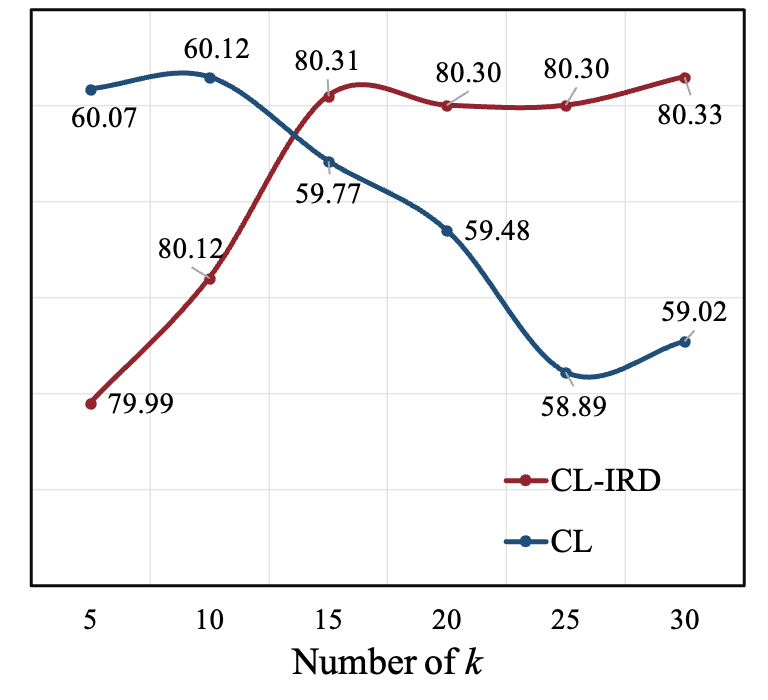
\includegraphics[width=0.9\hsize]{k.png}
%     \caption{Results with respect to different number of k.}
%     \label{fig:my_label}
% \end{figure}

